	\documentclass[journal]{IEEEtran}

\usepackage{cite}
\usepackage{amsmath,amssymb,amsfonts}
\usepackage{algorithmic}

\usepackage{graphicx}
\graphicspath{{../../Dissertacao/figuras/}}

\usepackage{textcomp}
\usepackage{xcolor}
\usepackage{booktabs}                        % AAB inserido
\usepackage[utf8]{inputenc}                  % AAB inserido
\usepackage{rotating}                        % AAB inserido

\usepackage{bm,bbm}
\usepackage[binary-units]{siunitx}

\usepackage[caption=false,font=footnotesize]{subfig}
\DeclareMathOperator{\traco}{tr}



\begin{document}
\title{Fusion of Evidences in Intensities Channels for Edge Detection in PolSAR Images}
\author{Anderson A.\ de Borba, Maurício Marengoni, and Alejandro C.\ Frery,~\IEEEmembership{Senior Member,~IEEE}%
\thanks{A.\ A.\ de Borba is with the Dept.\ Engenharia Elétrica e Computação, Universidade Presbiteriana Mackenzie (UPM), and with IBMEC-SP, São Paulo, Brazil. anderson.borba@ibmec.edu.br}
\thanks{M.\ Marengoni is with the Dept.\ Engenharia Elétrica e Computação,
UPM, São Paulo, Brazil. mauricio.marengoni@mackenzie.br}
\thanks{A.\ C.\ Frery is with the Laboratório de Computação Científica e Análise Numérica (LaCCAN), Universidade Federal de Alagoas (UFAL), Maceió, Brazil. acfrery@laccan.ufal.br}}

\maketitle

\begin{abstract}
Synthetic Polarimetric Aperture Radar (PolSAR) sensors have reached an essential position in the area of remote sensing. 
The images coming from PolSAR sensors have speckle noise, making their processing and analysis challenging tasks. 
The present study discusses a detection method based on the fusion of evidence obtained in the intensity (hh), (hv), and (vv) channels of PolSAR multi-look images. 
The method consists of detecting transition points in the thinnest range of data that covers two regions using the maximum likelihood with estimates parameters from the Wishart distribution. 
The fusion methods used are the simple average, the discrete wavelet (MR-DWT), and stationary (MR-SWT) transform with multi-resolution, the principal component analysis (PCA), the ROC statistic, and a multi-resolution method based on singular values (MR-SVD). 
The results indicate an assessment of the influence of each intensity channel in the fusion of evidence with possible paths for future research.
\end{abstract}

\begin{IEEEkeywords}
PolSAR, edge detection, maximum likelihood estimation, fusion methods. 
\end{IEEEkeywords}

\section{Introduction}\label{sec_01}
\IEEEPARstart{P}{olarimetric} synthetic aperture radar (PolSAR) has achieved an essential position as a remote sensing technology. 
The data such sensors provide require specifically tailored signal processing techniques.
Among such techniques, edge detection is one of the most important operations for extracting information.
Edges are at a higher level of abstraction than mere data and, as such, provide relevant insights about the scene.

Among the available edge detection techniques for SAR and PolSAR images, it is worth mentioning:
\begin{itemize}
\item techniques based on denoising~\cite{sjx, lzly, wxbzw, law, cgaf};   
\item Markov random fields~\cite{bf};	
\item the deep learning approach~\cite{bac, ztmxzxf} applied to segmentation and classification; and,
\item statistical techniques~\cite{gmbf, fbgm, nhfc} applied in edge detection in PolSAR / SAR imagery.
\end{itemize}

This article follows the statistical modeling approach using the techniques described in~\cite{gmbf, fbgm, nhfc} to find edge evidences, followed by fusion processes~\cite{mit, bmf_2019}. 
Our approach does not attempt to reduce the speckle, but to extract information from its statistical properties.

Instead of handling fully polarimetric data, we treat each intensity channel separately, obtain evidence of edges, and then produce a single estimator of the edge position.
With this, we quantify the contribution each channel provides to the solution of the problem.

We adopted the Gambini Algorithm~\cite{gmbf_sc}, which consists in casting rays and then finding the evidence of an edge in the ray by maximizing a value function.
The value function we use is the likelihood of two samples: one inside the edge, another outside the edge.
Without loss of generality, we assume the complex scaled Wishart distribution for the fully polarimetric observations~\cite{ade}, from which Gamma laws stem for each intensity channel.
The value function depends on the estimates that index such Gamma laws.
We estimate them by maximum likelihood with the BFGS optimization method implemented in the \texttt{maxLik} package~\cite{ht}.

The value function is the total likelihood.
It is non-differentiable at most points in the domain. 
It is known that classical methods have difficulties in finding the maximum of a non-differentiable functions. 
We used the Generalized Simulated Annealing (GenSA)~\cite{xgsh} method to solve this problem. 

We discuss six fusion methods:
\begin{itemize}
\item Simple average~\cite{mit}, 
\item Multi-Resolution Discrete Wavelet, MR-DWT~\cite{n_r},
\item Principal Component Analysis, PCA~\cite{n_r,mit},
\item ROC statistics~\cite{gs,fawcett},
\item Multi-Resolution Stationary Wavelet Transform, MR-SWT~\cite{n_r, jjly}, and 
\item Multi-Resolution Singular Value Decomposition, MR-SVD~\cite{naidu}.
\end{itemize}

It aims to show the feasibility of a procedure for edge detection in PolSAR images. 
The objective is to understand and quantify the importance of the information provided by each channel to improve the edge detection process.

The article is structured as follows.
Section~\ref{sec_02} describes statistical modeling.
Section~\ref{sec_03} describes edge detection for PolSAR data.
Section~\ref{sec_04} describes the approach to edge evidence fusing.
Section~\ref{sec_05} presents numerical results.
Finally, Section~\ref{sec_06} concludes the work with observations, future directions of research, and the feasibility of detecting edges in each channel of PolSAR images.

\section{Statistical modeling for PolSAR data}\label{sec_02}

Multi-looked fully polarimetric data follow the Wishart distribution with PDF defined by:
\begin{equation}
    f_{\mathbf{Z}}(\mathbf{Z};\mathbf{\Sigma},L)=\frac{L^{mL}|\mathbf{Z}|^{L-m}}{|\mathbf{\Sigma}|^{L}\Gamma_m(L)} \exp(-L\traco(\mathbf{\Sigma}^{-1}\mathbf{Z})),
    \label{eq:DistWishart}
\end{equation} 
where, $\traco(\cdot)$ is the trace operator of a matrix, $\Gamma_m(L)$ is the multivariate Gamma function defined by $
	\Gamma_m(L)=\pi^{\frac{1}{2}m(m-1)} \prod_{i=0}^{m-1}\Gamma(L-i)$,
and $\Gamma(\cdot)$ is the Gamma function.
We used three $m=3$ channels in this study. 
This situation is denoted by $\mathbf{Z}\sim W(\mathbf{\Sigma}, L)$, which satisfies $E[\mathbf{Z}]=\mathbf{\Sigma}$. 
This assumption usually holds on targets where the speckle is fully developed but, since we will estimate $L$ on each sample (instead of considering the same number of looks for the whole image), we will in part take into account departures from such hypothesis.

Fully polarimetric data may be modeled by~\eqref{eq:DistWishart}.
Since we are interested in describing the information conveyed by parts of such matrix, we rely on the results presented in~\cite{lee,hsbmp}.
In particular, we assume that the distribution of each intensity channel is a 
Gamma law with probability density function
\begin{equation}
f_Z(z;\mu,L)=\frac{L^{L}z^{L-1}}{\mu^{L}\Gamma(L)} \exp\big\{-Lz/\mu\big\},\quad z>0,
\label{func_dens_uni_gamma}
\end{equation}
where $L>0$ (rather than $L\geq1$ to allow for flexibility), and
$\mu>0$ is the mean.

Given the sample $\bm z = (z_1,\dots,z_n)$,
the reduced log-likelihood of this model is
\begin{equation}
\ell(\bm z; L,\mu) = 
n \big[L\ln (L / \mu) - \ln \Gamma(L)\big]
+L \sum_{k=1}^{n}\ln z_k -\frac{L}{\mu}\sum_{k=1}^{n} z_k.
\label{eq:LogLikelihoodGamma}
\end{equation}

We obtain $(\widehat L, \widehat \mu)$, the maximum likelihood estimator (MLE) of $(L, \mu)$ based on $\bm z$, by maximizing~\eqref{eq:LogLikelihoodGamma} with the BFGS method implemented in the \texttt{maxLik} package~\cite{ht}.
We prefer optimization to solving $\nabla\ell=\bm 0$ for improved numerical stability.

\section{Edge Detection on a Single Data Strip}\label{sec_03}

We approach edge detection with the Gambini Algorithm~\cite{gmbf, fbgm, nhfc}.
%%% ACF
%This technique is convenient for our subsequent fusion step, since it provides estimates of the edge location over the same ray.
It consists of the following steps:
\begin{enumerate}
	\item Identify the centroid of a region of interest (ROI) in an automatic, semi-automatic or manual manner.
	\item Cast rays from the centroid to the outside of the area.
	\item Collect data on a strip, ideally of the size of a pixel, around the rays using the  Bresenham's midpoint line algorithm.
	\item Compute the value function on every point of the ray.
	\item Use the GenSA method~\cite{xgsh}, to find points of maxima in the functions of interest.
	\item Fuse the evidence of detected edges in the (hh), (hv) and (vv) channels.
\end{enumerate}

The value function is the reduced log-likelihood of the inner and external samples of the strip denoted, respectively, as $\bm z_\text{I}$ and $\bm z_\text{E}$.
Each strip $z = (z_1,z_2,\dots,z_n)$ is, thus, partitioned in two disjoint samples at position $j$:
$$
z = (\underbrace{z_1,z_2,\dots,z_j}_{\bm z_\text{I}}, 
\underbrace{z_{j+1}, z_{j+2},\dots,z_n}_{\bm z_\text{E}}).
$$
We assume two (possibly) different models for each partition:
$\bm Z_\text{I} \sim \Gamma(\mu_\text{I},L_\text{I})$, and 
$\bm Z_\text{E} \sim \Gamma(\mu_\text{E},L_\text{E})$.
We then estimate $(\mu_\text{I},L_\text{I})$ and $(\mu_\text{E},L_\text{E})$ with $\bm z_\text{I}$ and $\bm z_\text{E}$, respectively, by maximizing~\eqref{eq:LogLikelihoodGamma}, and obtain $(\widehat{\mu}_\text{I}, \widehat{L}_\text{I})$ and $(\widehat{\mu}_\text{E}, \widehat{L}_\text{E})$.

The total log-likelihood at point $j$ is, then,
\begin{equation}\label{eq:TotalLogLikelihood}
\begin{split}
%\ell(j&;\bm z_\text{I},\bm z_\text{E}) = \\
\ell(j&;\widehat{\mu}_I, \widehat{L}_I,\widehat{\mu}_E, \widehat{L}_E)=\\
&j \big[\widehat{L}_\text{I}\ln (\widehat{L}_\text{I} / \widehat{\mu}_\text{I}) - \ln \Gamma(\widehat{L}_\text{I})\big]
+\widehat{L}_\text{I} \sum_{k=1}^{j}\ln z_k -\frac{\widehat{L}_\text{I}}{\widehat{\mu}_\text{I}}\sum_{k=1}^{j} z_k +\\
&(n-j) \big[\widehat{L}_\text{E}\ln (\widehat{L}_\text{E} / \widehat{\mu}_\text{E}) - \ln \Gamma(\widehat{L}_\text{E})\big]
+\widehat{L}_\text{E} \sum_{k=j+1}^{n}\ln z_k -\\ &\frac{\widehat{L}_\text{E}}{\widehat{\mu}_\text{E}}\sum_{k=j+1}^{n} z_k.
\raisetag{2.2em}
\end{split}
\end{equation}
We then apply GenSA to find  
$$
\widehat{\jmath}= \arg\max\limits_{j\in [\min_s,N-\min_s]}\ell(j;\widehat{\mu}_I, \widehat{L}_I,\widehat{\mu}_E, \widehat{L}_E),
$$ 
where $\min_s$ is a minimum sample size that we set to $14$.

In this way, we obtain one estimates for the edge for each intensity channel.
Notice that this approach can be extended and/or modified to cope with any kind of data.

We will see ways of fusing these evidences in the next section.

\section{Fusion of Evidences}\label{sec_04}

Denote in the following $\widehat{\bm\jmath}_c$ the binary image with same support as the input data $c$ ($m$ lines and $n$ columns; denote $\ell=mn$), where $1$ denotes an estimate of edge and $0$ otherwise.
We have $n_c$ of these image to fuse, and the result of the fusion will be denoted $\bm I_F$.

We compare the results of six fusion techniques, namely:
simple average, 
multi-resolution discrete wavelet transform (MR-DWT),
principal components analysis (PCA), 
ROC statistics,
multi-resolution stationary wavelet transform (MR-SWT), and
multi-resolution singular value decomposition (MR-SVD).

%The estimated evidence image and the fusion image are defined to perform the fusion techniques. The first can be defined as $\widehat\jmath_c(x,y)$, where $x$ and $y$, indicate the range of pixels in an image equal in size to the data image chosen for analysis. The image is binary, where the value one is put on the pixel estimated as edge evidence by the MLE method, and zero on the other pixels, for each channel. The second called $\text{I}_F(x,y)$ is the result of the fusion method. 

%Refs.~\cite{bmf_2019,n_r,mit,gs,fawcett} provide details about the three first.
%We describe the two latter below.

\subsection{Simple Average}
The simple average fusion method proposes the arithmetic mean of the edge evidence in each of the $n_c$ channels:
$\bm I_F(x,y)=(n_c)^{-1}\sum_{c=1}^{n_c} \widehat{\bm\jmath}_c(x,y)$.
%where $\widehat\jmath_c$ denotes the estimate obtained in channel $c$.

\subsection{Multi-Resolution Discrete Wavelet -- MR-DWT} 
This section is based on~\cite{n_r}.
%We apply DWT filters separately in the vertical and horizontal directions of each image $\bm{\widehat\jmath}_c$, then down-sampled by a factor of two. 
%In this way, each image is filtered by the low pass filter $\text{L}$ in the vertical direction and the high pass filter $\text{H}$ in the horizontal direction, then down-sampled to create the matrices coefficients  $\bm{\widehat\jmath}_{c\text{L}}$ and $\bm{\widehat\jmath}_{c\text{H}}$.
We apply DWT filters on each binary image $\bm{\widehat\jmath}_c$: a low-pass filter $\bm L$ in the vertical direction, and a high-pass filter $\bm H$ in the horizontal direction, then both are down-sampled to create the coefficient matrices $\bm{\widehat\jmath}_{c\text{L}}$ and $\bm{\widehat\jmath}_{c\text{H}}$.
These operations are repeated on the coefficient matrices, leading to $\bm{\widehat\jmath}_{c\text{LL}}$, $\bm{\widehat\jmath}_{c\text{LH}}$, $\bm{\widehat\jmath}_{c\text{HL}}$, and $\bm{\widehat\jmath}_{c\text{HH}}$.

%%% ACF Detalhar as operações usando a notação acima: a média é pixel-a-pixel? quais bandas são promediadas?
%%% AAB A média é pixel a pixel. Todas as bandas são usadas na média. Vou tentar deixar claro no texto. Creio que respondi no item 2 abaixo.
%%% AAB Eu entendo que investigar outros tipo de ponderação (suprimir canais, por exemplo) pode ser realizado. Ainda não consegui fazer esses testes.
%%% AAB O nivel de resolução que uso é 1, esse é outro ponto de investigação, seria interessante aumentar esse nível e ver o que acontece na fusão. Tb não consegui realizar esses teste. Inseri no item 1) abaixo a info sobre o nível de resolução.
The DWT fusion method has the following steps:
\begin{enumerate}
\item Calculate the DWT decomposition $\bm{\widehat\jmath}_{c\text{LL}}$, $\bm{\widehat\jmath}_{c\text{LH}}$, $\bm{\widehat\jmath}_{c\text{HL}}$, and $\bm{\widehat\jmath}_{c\text{HH}}$, for each channel.
\item Compute $\bm{\bar\jmath}_{c\text{HH}}$, the pixel-wise mean of all $\bm{\widehat\jmath}_{c\text{HH}}$ decompositions.
\item Find the pixel-wise maximum of $\bm{\widehat\jmath}_{c\text{LL}}$, $\bm{\widehat\jmath}_{c\text{LH}}$, $\bm{\widehat\jmath}_{c\text{HL}}$: $\bm{\bar\jmath}_{c\text{LL}}$, $\bm{\bar\jmath}_{c\text{LH}}$, and $\bm{\bar\jmath}_{c\text{HL}}$.
%%% AAB(03/03/2020) tenho uma dúvida, o máximo(pixel a pixel) deve ser calculada entre os operadores da decomposiçcao em cada canal. Não seria bom deixar claro como no item anterior?
\item The result of the fusion $\text{I}_F$ is the inverse DWT transformation of the coefficient matrices $\bm{\bar\jmath}_{c\text{HH}}$, $\bm{\bar\jmath}_{c\text{LL}}$, $\bm{\bar\jmath}_{c\text{LH}}$, and $\bm{\bar\jmath}_{c\text{HL}}$.
\end{enumerate}
%%% ACF Aqui dizer que é a Inverse DWT do que
\subsection{Principal Component Analysis -- PCA}

%%% ACF Revisar e corrigir a notação; usar notação matemática sempre que necessário
This section is based on~\cite{n_r,mit}.
The method is comprised of the following steps:
\begin{enumerate}
\item Stack the binary images $\bm{\widehat\jmath}_c$ in column vectors to obtain the matrix $\bm X_{\ell\times n_c}$.
%\item Calculate the average of the elements of these columns, generating a vector of dimension of $1\times nc$.
%%% ACF A matriz de covariância é invariante a traslações. Precisa deste passo?
%\item subtract the average of each column from $\text Y$, resulting in a matrix of the same dimension of $\text X$; 
\item Calculate the covariance matrix $\bm C_{n_c\times n_c}$ of $\bm X_{\ell\times n_c}$.
\item Compute the matrices of eigenvalues ($\bm\Lambda$) and eigenvectors ($\bm V$) of the covariance matrix, sorted in decreasing order by the eigenvalues. %The matrices generated by the eigenvalues, on the principal diagonal, and the eigenvectors placed in columns;
%%% ACF O que é V_c?
\item Compute the components $\bm P_c=(\sum_{m=1}^{n_c} \bm V_c(m))^{-1}{\bm V_c}$, where $\bm V_c$ is eigenvector associated with the highest eigenvalue of $\bm X$; notice that $\sum_{c=1}^{n_c}\bm P_c=1$.
\item Fuse $\bm I_F(x,y)=\sum_{c=1}^{n_c}\bm P_c\bm{\widehat\jmath}_c(x,y)$.
\end{enumerate}

\subsection{ROC Statistics}
The ROC method was proposed and described on~\cite{gs,fawcett}:
\begin{enumerate}
%\item the evidence of edges in each channels $\bm{\widehat\jmath}_c$, with $c=1,\dots,nc$ in a binary way;
%%% AAB(03/03/2020) Aqui fico em dúvida se coloco "matrices" ou  "binary images".  
\item Add the binary images $\bm{\widehat\jmath}_c$ to produce the frequency matrix ($\bm V$).
\item Use thresholds ranging from $t=1,\dots,n_c$ on $\bm V$ to generate matrices $\bm M_t$.
\item Compare each $\bm M_t$ with all $\bm{\widehat\jmath}_c$, find the confusion matrix to generate the ROC curve. 
The optimal threshold corresponds to the point of the ROC curve closest (in the sense of the Euclidean distance) to the diagnostic line.
\item The fusion $\bm I_F$ is the matrix $\bm M_t$ which corresponds to the optimal threshold.
\end{enumerate}

\subsection{Multi-Resolution Stationary Wavelet Transform -- MR-SWT}  
This section is based on~\cite{n_r, jjly}. The difference between MR-DWT and MR-SWT method is the replacement of the method discrete wavelet transform (DWT) by the method stationary wavelet transform SWT. 
%%% ACF Esclarecer quais são estes filtros

\subsection{Multi-Resolution Singular Value Decomposition -- MR-SVD}

MR-SVD Fusion~\cite{naidu} works similarly to MR-DWT. 
The difference consists in changing the DWT filters by the SVD filters. 
The MR-SVD fusion method can be summarized as follows:
\begin{enumerate}
%\item Organize the binary image $\bm{\widehat\jmath}_c$ in matrices $\text{X}_\ell$ with dimension $4\times\frac{\text{M}}{2}\frac{\text{N}}{2}$ according to~\cite{naidu}, where M is the number of rows and N is the number of columns in $\bm{\widehat\jmath}_c$, and $\ell$ is the level resolution to set. In this work is used one resolution level;
\item Organize the binary image $\bm{\widehat\jmath}_c$ as non-overlapping $2\times 2$ blocks, and arrange each block as a $4\times 1$ vector by stacking columns to form the data matrix $\bm X_1$.
%, where M is the number of rows and N is the number of columns in $\bm{\widehat\jmath}_c$, 
%and $\ell$ is the level resolution to set. In this work is used one resolution level.
%%% ACF Repare que não usou M nem N
\item Find the SVD decomposition of $\bm X_1$, and calculate $\bm T_1=\bm X_1 \bm X_1^T=\bm U_1 \bm S_1^2 \bm U_1^T$, where $s(1)\geq s(2) \geq s(3) \geq s(4)$ compose the singular value matrix $\bm S_1$, 
%%% ACF Não definiu nem usou s(1), s(2) etc
%%% AAB Os s(1), s(2), s(3) e s(4) são usados para gerar a matriz $S$
 and $\bm U_1$ is unitary.
\item 
Transform the lines of $\widehat{\bm X}_1=\bm U_1^T\bm X_1$ into new matrices with dimensions $\frac{m}{2}\times\frac{n}{2}$: $\{\bm\Phi_1, \bm\Psi_1^\text{V}, \bm\Psi_1^\text{H}, \bm\Psi_1^\text{D}\}$. 
%\item Repeat the procedure on $\Phi_r$ $R$ times. Where $r=1,\dots,\text{R}$ and, R is lowest resolution index. 
\item Repeat the procedure on $\bm\Phi_r$. Where $r=1,\dots,\text{R}$ and, R is lowest resolution index. 
\item The MR-SVD method is represented as
\begin{equation}\label{msvd_iter}
\widehat{\bm X}\leftarrow \left\{\bm \Phi_\text{R},\{\bm\Psi_r^\text{V},\bm\Psi_r^\text{H},\bm\Psi_r^\text{D} \}_{r=1}^\text{R},\{\bm U_r\}_{r=1}^\text{R} \right\}.
\end{equation}
%\item Once the SVD is applied to level $\ell$ the fusion process is executed as follow: In the operators $\Psi_\ell^\text{V}$, $\Psi_\ell^\text{H}$ and $\Psi_\ell^\text{D}$, the maximum is found among all channel, pixel by pixel, resulting in new operators $\bar{\Psi}_\ell^\text{V}$, $\bar{\Psi}_\ell^\text{H}$ and $\bar{\Psi}_\ell^\text{D}$. 
%The operators $\Phi_L$, and $\text{U}_\ell$ are averaged over all the channels, pixel by pixel.
\item Once decomposition is applied to all channels.
\item Compute $\overline{\bm\Phi}_\text{R}$ averaged $\bm\Phi_R$, and $\overline{\bm U}_r$ averaged $\bm U_r$ decompositions.
\item Find the pixel-wise maximum of $\bm\Psi_r^\text{V}$, $\bm\Psi_r^\text{H}$ and $\bm\Psi_r^\text{D}$ : $\overline{\bm\Psi}_r^\text{V}$, $\overline{\bm\Psi}_r^\text{H}$ and $\overline{\bm\Psi}_r^\text{D}$ .
\item The fusion $\bm I_F(x,y)$ is the SVD transformation to $\overline{\bm\Phi}_R$, $\overline{\bm U}_r$, $\overline{\bm\Psi}_r^\text{V}$, $\overline{\bm\Psi}_r^\text{H}$ and $\overline{\bm\Psi}_r^\text{D}$,  for each level $r=1,\dots,\text{R}$. 
\end{enumerate}

\section{Results}\label{sec_05}

\subsection{PolSAR image}

We used a $750\times 1024$ pixels AIRSAR PolSAR image of Flevoland, L-band, for the tests. 
Fig.~(\ref{flevoland_radial_4look}) shows the ROI, with the radial lines where edges are detected. 

\begin{figure}[hbt]
\centering
	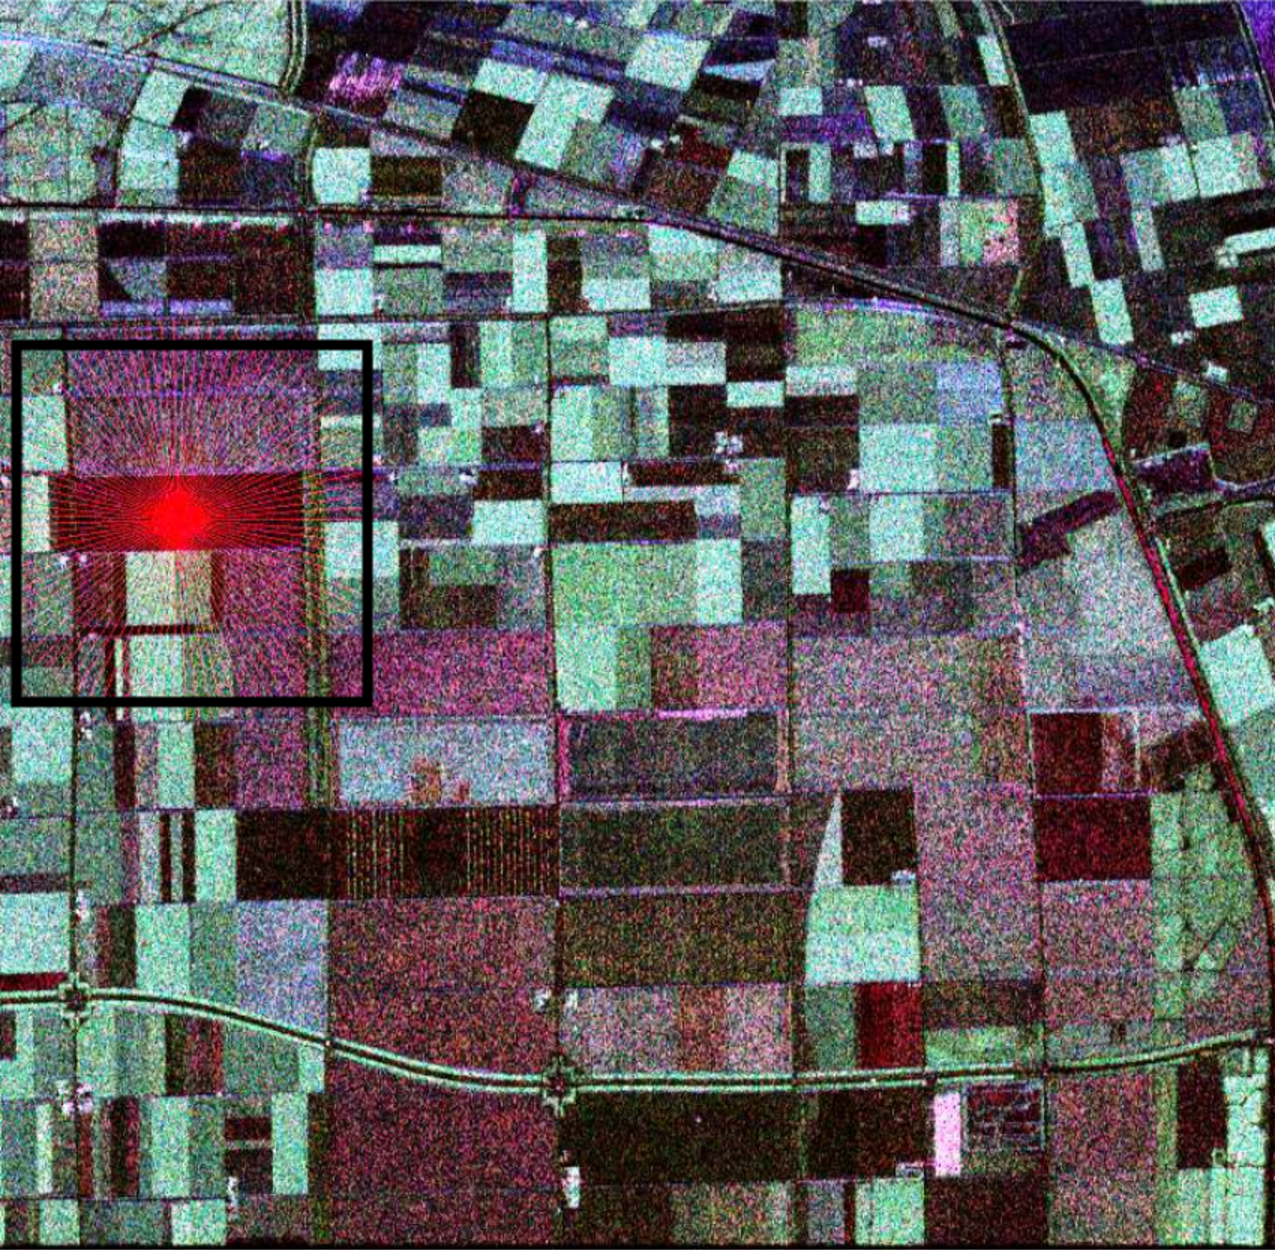
\includegraphics[width=\linewidth]{flevoland_radial_4_look_black}
	\caption{Flevoland image in Pauli decomposition, with Region of Interest (ROI) and rays.}
\label{flevoland_radial_4look}
\end{figure}

%The estimates from equation~\eqref{eq:LogLikelihoodGamma} is used in equation~\eqref{eq:TotalLogLikelihood} generating an oscillation at the end of each radial line, depending on the radial considered. In order to get around this problem, in this PolSAR image, 14 pixels on each side of radial lines were not considered. The number of pixel were determined empirically.

Figs.~\ref{evidencias_hh_hv_vv}\subref{evidencias_hh_hv_vv:a}, \subref{evidencias_hh_hv_vv:b} and~\subref{evidencias_hh_hv_vv:c} show, respectively, the edge evidence in the $\text{hh}$, $\text{hv}$ and $\text{vv}$ channels as obtained by MLE.

It is worth noting that GenSA has accurately identified the maximum value of function $\ell(j)$, even in the presence of multiple local maxima. 
A visual assessment leads to conclude that the best results are provided by the $\text{hv}$, although with a few points far from the actual edge.

   \begin{figure*}[hbt]
	\centering
     \subfloat[Evidences in channel $\text{hh}$ \label{evidencias_hh_hv_vv:a}]{%
       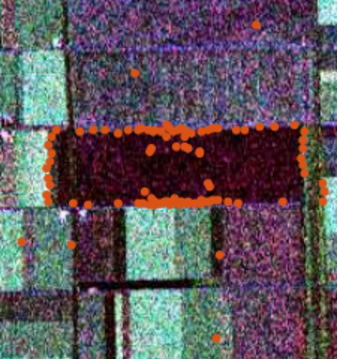
\includegraphics[width=0.32\linewidth]{flevoland_hh_evid_param_L_mu_14_pixel_crop}
     }
     \subfloat[Evidences in channel $\text{hv}$ \label{evidencias_hh_hv_vv:b}]{%
       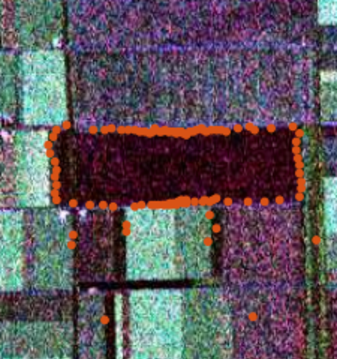
\includegraphics[width=0.32\linewidth]{flevoland_hv_evid_param_L_mu_14_pixel_crop}
     }
     \subfloat[Evidences in channel $\text{vv}$ \label{evidencias_hh_hv_vv:c}]{%
       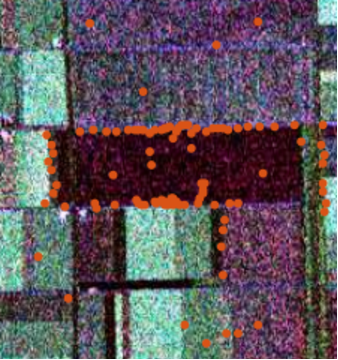
\includegraphics[width=0.32\linewidth]{flevoland_vv_evid_param_L_mu_14_pixel_crop}
     }
     \caption{Edges evidences from the three intensity channels}
     \label{evidencias_hh_hv_vv} 
   \end{figure*}

Figs.~\ref{fusion_met}\subref{fusion_met:a}, \subref{fusion_met:b}, \subref{fusion_met:c}, \subref{fusion_met:d}, \subref{fusion_met:e}, and~\subref{fusion_met:f} show the results of fusing these evidences. 
Table~\ref{metrica_de_tempo} shows the running times (absolute and relative to the fastest method).

%Thus, one can see that the time for the PCA method is 2.19 times longer than the simple average.  

The simple average and PCA produce similar results.
MR-SVD produces considerably less outliers than the other methods, at the cost of longer processing time.
ROC produces accurate edges, with few outliers, but sparsely. 
%One way to get around this problem would be to increase the number of channels considered using other PDF.
Both wavelet-based methods (DWT and SWT) produce too dense edges and many outliers.

%The post-processing is an option to be used in all the fusion methods. 
%An idea can be found in Ref.~\cite{fbgm}. 

\begin{figure*}[hbt]
	\centering
     \subfloat[Average fusion\label{fusion_met:a}]{%
       %\includegraphics[width=0.2\textwidth]{example-image-a}
       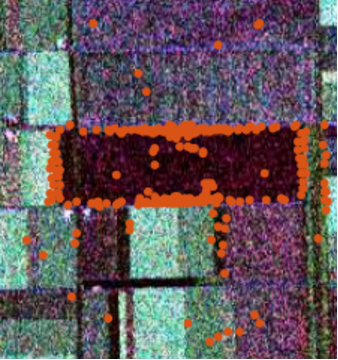
\includegraphics[width=0.32\linewidth]{flevoland_fus_media_param_L_mu_14_pixel_crop}
     }
     \subfloat[DWT fusion\label{fusion_met:b}]{%
       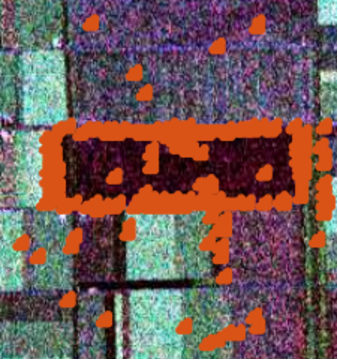
\includegraphics[width=0.32\linewidth]{flevoland_fus_dwt_param_L_mu_14_pixel_crop}
     }
     \subfloat[PCA fusion \label{fusion_met:c}]{%
       %\includegraphics[width=0.2\textwidth]{example-image-a}
       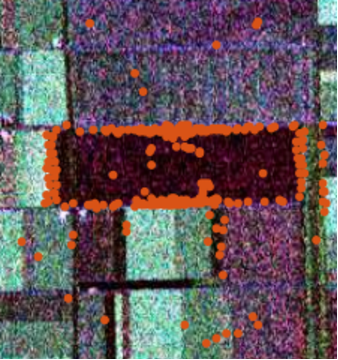
\includegraphics[width=0.32\linewidth]{flevoland_fus_pca_param_L_mu_14_pixel_crop}       
     }\\
     \subfloat[ROC fusion\label{fusion_met:d}]{%
       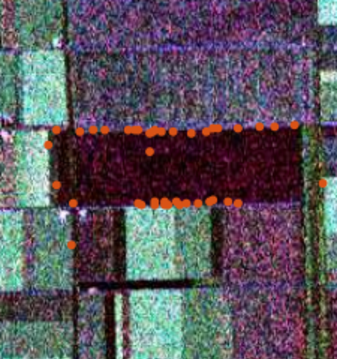
\includegraphics[width=0.32\linewidth]{flevoland_fus_roc_param_L_mu_14_pixel_crop}
     }
     \subfloat[MR-SWT fusion\label{fusion_met:e}]{%
       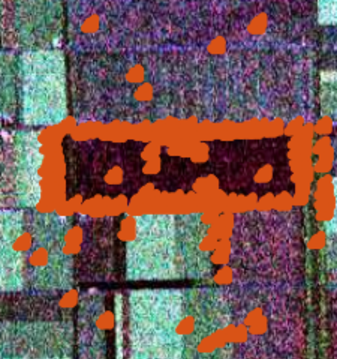
\includegraphics[width=0.32\linewidth]{flevoland_fus_swt_param_L_mu_14_pixel_crop}
     }
     \subfloat[MR-SVD fusion\label{fusion_met:f}]{%
       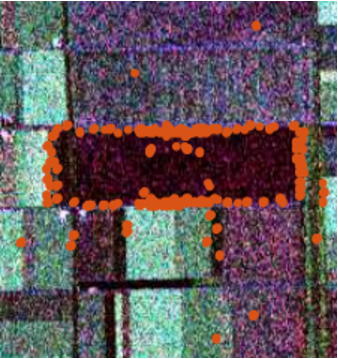
\includegraphics[width=0.32\linewidth]{flevoland_fus_svd_param_L_mu_14_pixel_crop}
     }
     \caption{Results of applying the six fusion methods}
     \label{fusion_met}
\end{figure*}

\subsection{Processing times} 

The processing times reported in Table~\ref{metrica_de_tempo} are the average of $20$ runs, measuring only the fusion step.
%\begin{table}[hbt]
%	\centering
%	\tiny
%	\caption{Processing times (fusion method).}\label{metrica_de_tempo}
%	\begin{tabular}{@{}lrrrrrr@{}} \toprule
%		Method       & Average    &   PCA      &  ROC      & MR-DWT   &  MR-SWT        &  MR-SVD \\ \midrule
%		Time (s)      & 0.01      &  0.02      &0.40       &0.08      &  0.18 & 1.11  \\
%		Rel. time     & 1.00      & 2.19       &46.59      & 9.25     & 21.05 & 129.57  \\ \bottomrule
%	\end{tabular}
%\end{table}
%
\begin{table}[hbt]
	\centering
	\caption{Processing times (fusion method).}\label{metrica_de_tempo}
	\begin{tabular}{@{}lrrrrrr@{}} \toprule
		Method       & Aver   &   PCA      &  MR-DWT  & MR-SWT &  ROC  &  MR-SVD \\ \midrule
		Time (s)      & 0.01      & 0.02       &  0.08 & 0.18      &  0.40       & 1.11  \\
		Rel. time     & 1.00      & 2.19       &  9.25 & 21.05     &  46.59      & 129.57  \\ \bottomrule
	\end{tabular}
\end{table}

\subsection{Implementation Details}

The system presented here was executed on a Intel\copyright\ Core i7-9750HQ CPU \SI{2.6}{\giga\hertz} \SI{16}{\giga\byte} RAM computer.  
The method for detecting edge evidence MLE was implemented in the R language.
The fusion methods were implemented in Matlab. 


\section{Conclusion}\label{sec_06}

We found evidence of edges using the maximum likelihood method under the Wishart model for PolSAR data. 
The evidence was found in each of the three intensity channels of an AIRSAR L-band image over Flevoland.

The best edge evidence was observed on the hv channel.

We applied simple average, MR-DWT, PCA, ROC, MR-SWT, and MR-SVD fusion methods to aggregate the evidence obtained in the three channels.
The best results, from a visual standpoint, were produced by the Multi-Resolution Singular Value Decomposition (MR-SVD), at the cost of the highest processing time.
We assessed the results by checking the closeness of the fused points to the actual edge, by the presence of outliers, and by the blurring effect.

We highlight two avenues for future improvement of the fusion:
\begin{enumerate}
	\item increasing the number of evidences.
	This is possible, since fully polarimetric data is richer than mere intensity channels; and
	\item post-processing both the partial evidences and the fusion.
\end{enumerate}

\bibliographystyle{IEEEtran}
\bibliography{../../../Text/bibliografia}
\end{document}

